\documentclass[12pt]{article}

\usepackage{HWStyle_OWEN}

\newcommand{\hmwkClass}{Numerical Analysis}
\newcommand{\hmwkAuthorName}{Aoyang Yu (3190102166)}
\newcommand{\hmwkTitle}{Homework \#3}

\begin{document}

\maketitle

\section{Programming Assignments}

    \subsection{A}

        See the design document.
    
    \subsection{B}

        The max-norm of the errors are listed in the following table.
        \begin{table}[H]
            \centering
            \begin{tabular}{c | c c}
                \(N\) & complete & not-a-knot \\
                \hline
                5 &  \(4.21705\times 10^{-1}\) & \(4.31538\times 10^{-1}\) \\
                10 & \(2.05289\times 10^{-2}\) & \(2.05334\times 10^{-2}\) \\ 
                20 & \(3.16894\times 10^{-3}\) & \(3.16894\times 10^{-3}\) \\
                40 & \(2.75356\times 10^{-4}\) & \(2.75356\times 10^{-4}\) \\
                80 & \(1.60900\times 10^{-5}\) & \(1.60900\times 10^{-5}\) \\
            \end{tabular}
        \end{table}
        The rates of convergence are estimated as follows.
        \begin{table}[H]
            \centering
            \begin{tabular}{c c}
                complete & not-a-knot \\
                3.483 & 3.489
            \end{tabular}
        \end{table}
        The interpolations are plotted.
        \begin{figure}[H]
            \centering
            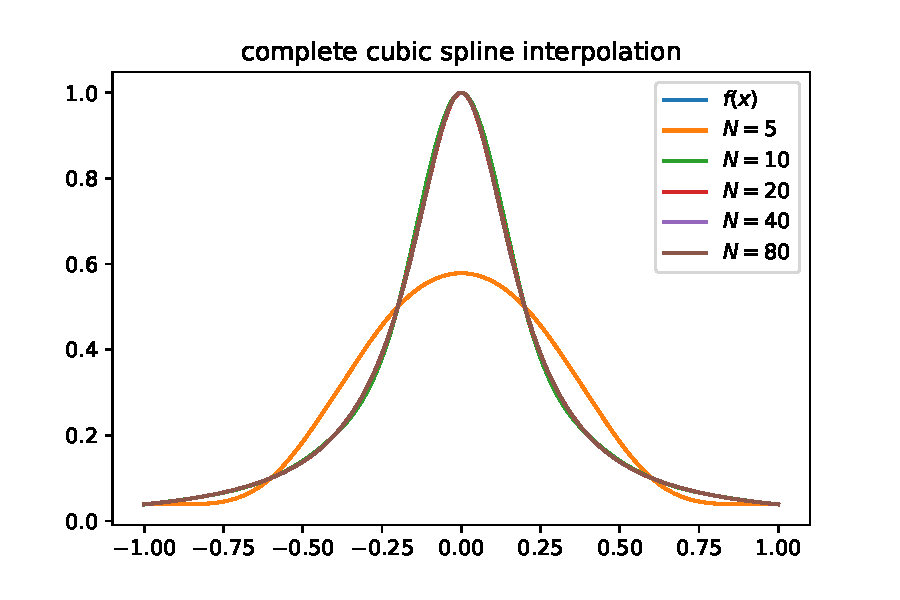
\includegraphics{pics/B_complete}
        \end{figure}
        \begin{figure}[H]
            \centering
            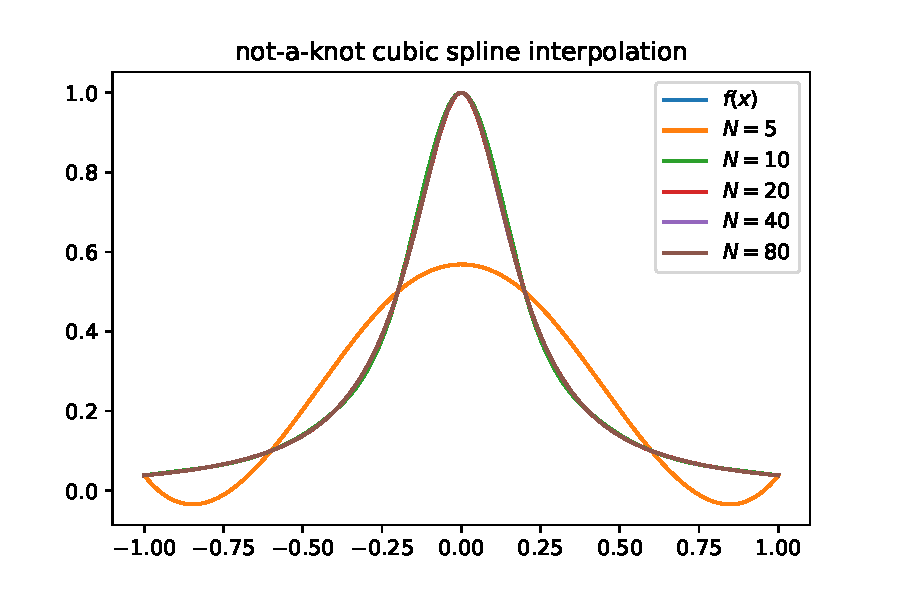
\includegraphics{pics/B_notAknot}
        \end{figure}

    \subsection{C}

        The following is the plot.
        \begin{figure}[H]
            \centering
            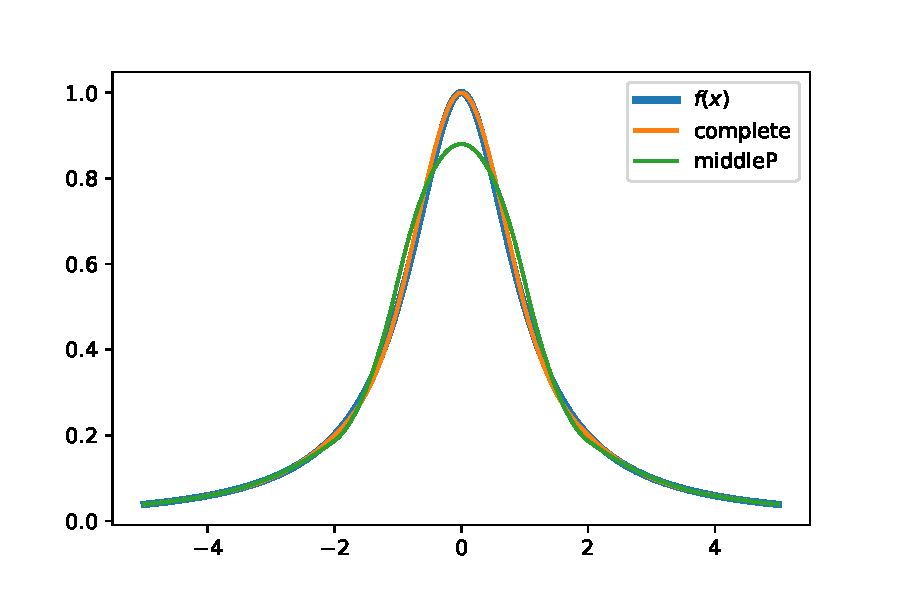
\includegraphics{pics/C}
        \end{figure}

    \subsection{D}

        The errors are listed in the following table.
        \begin{table}[H]
            \centering
            \begin{tabular}{c | c c}
                \(x\) & \(E_\text{complete}\) & \(E_\text{middleP}\) \\
                \hline
                \(-3.50\) & \(6.6957\times 10^{-4}\) & \(0.0000\times 10^{0}\) \\
                \(-3.00\) & \(0.0000\times 10^{0}\) & \(1.4184\times 10^{-3}\) \\
                \(-0.50\) & \(2.0529\times 10^{-2}\) & \(1.1102\times 10^{-16}\) \\
                \(0.00\) & \(1.1102\times 10^{-16}\) & \(1.2024\times 10^{-1}\) \\
                \(0.50\) & \(2.0529\times 10^{-2}\) & \(1.1102\times 10^{-16}\) \\
                \(3.00\) & \(0.0000\times 10^{0}\) & \(1.4184\times 10^{-3}\) \\
                \(3.50\) & \(6.6957\times 10^{-4}\) & \(0.0000\times 10^{0}\) \\
            \end{tabular}
        \end{table}

        Some errors are close to the machine precision, because by the
        interpolation conditions, the spline should match exactly with the exact function.
        Therefore, mathematically the error is \(0\), and computationally the 
        error should be close to machine precision.

        The accuracies of the two splines differ at different points. In general, 
        the complete B-spline is more accurate at approximating points, i.e., points
        not in the interpolation conditions.

    \subsection{E}

        First, to get an understanding of the curve, I picked some points 
        on it and scatter-plotted them. I found that the \textbf{critical points} are
        those with \(x=0\) and \(x=\pm \sqrt 3\). I also decided to \textbf{use two pieces of spline} to
        plot the curve, one for the left half and one for the right half. They are symmetric 
        so practically I only need to calculate the right half. By examing the property of
        the curve when \(x\to 0^+\), I found that locally the curve looks like a vertical line, 
        which means that \(x'(t_0)=0\). So I think we should pose constraints on the first 
        derivative of the spline at endpoints, which means the \textbf{complete spline condition} 
        is appropriate.

        The three plots are listed below, with blue points indicating the sample points and
        the red curve is our spline.

        \begin{figure}[H]
            \centering
            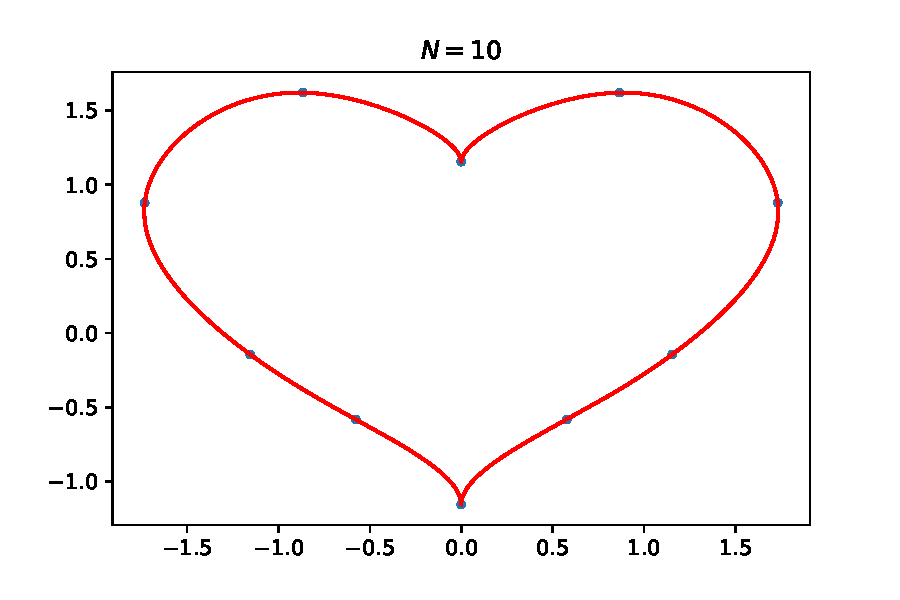
\includegraphics{pics/E_10}
        \end{figure}
        \begin{figure}[H]
            \centering
            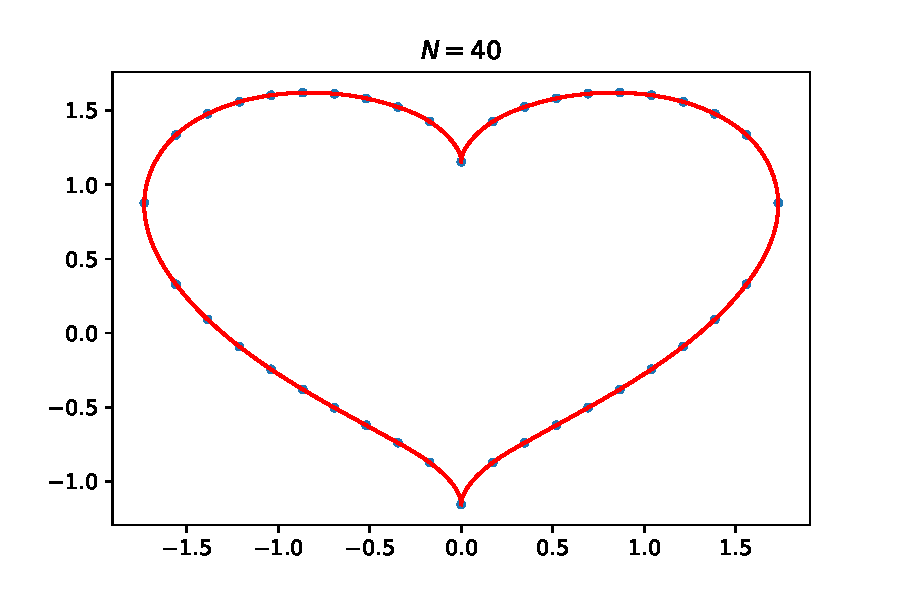
\includegraphics{pics/E_40}
        \end{figure}
        \begin{figure}[H]
            \centering
            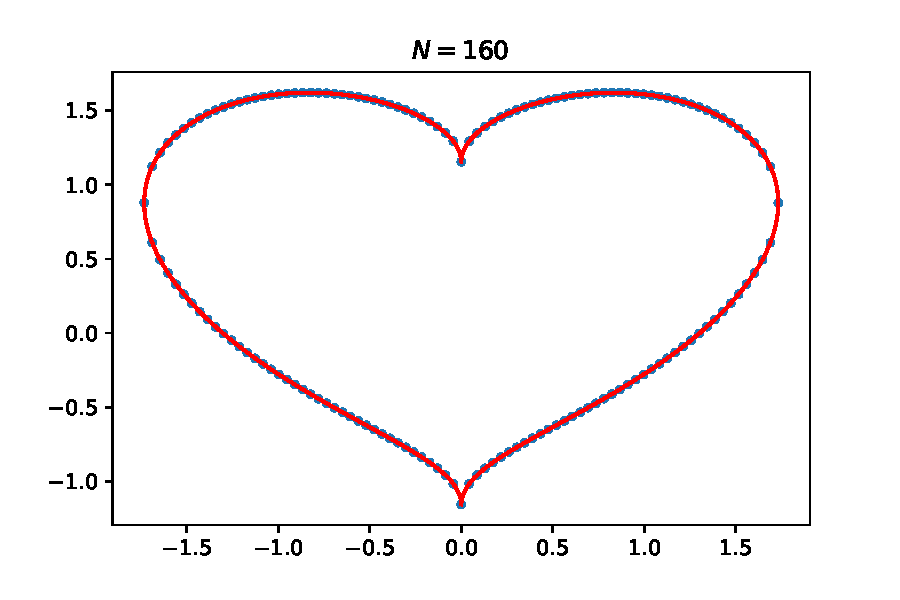
\includegraphics{pics/E_160}
        \end{figure}

    \subsection{F}

        My construction of the three splines are plotted below.
        \begin{figure}[H]
            \centering
            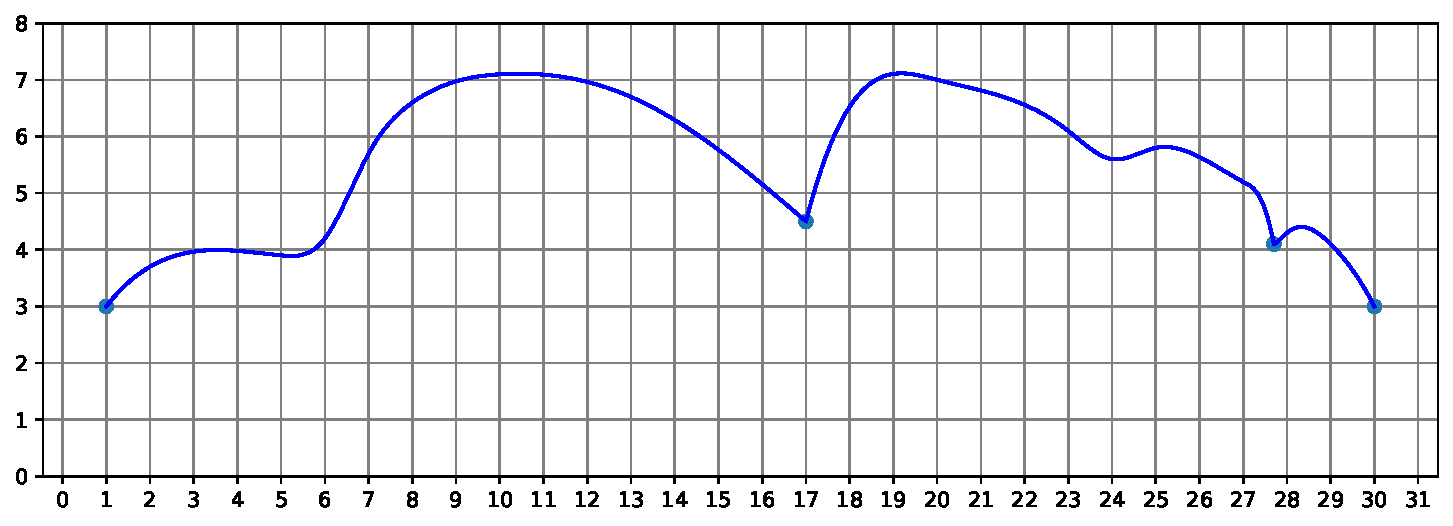
\includegraphics[scale=0.64]{pics/F}
        \end{figure}

    \subsection{G}
        
        \(n=1\)
        \begin{figure}[H]
            \centering
            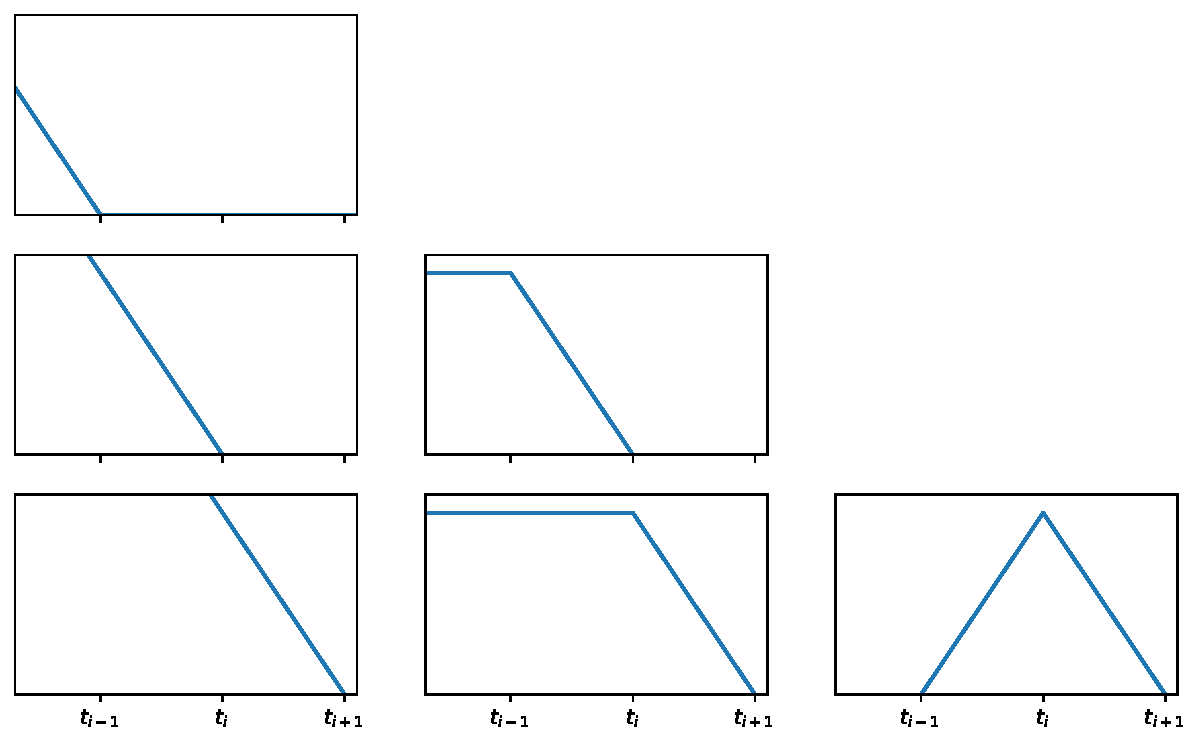
\includegraphics[scale=0.8]{pics/G_1}
        \end{figure}
        \(n=2\)
        \begin{figure}[H]
            \centering
            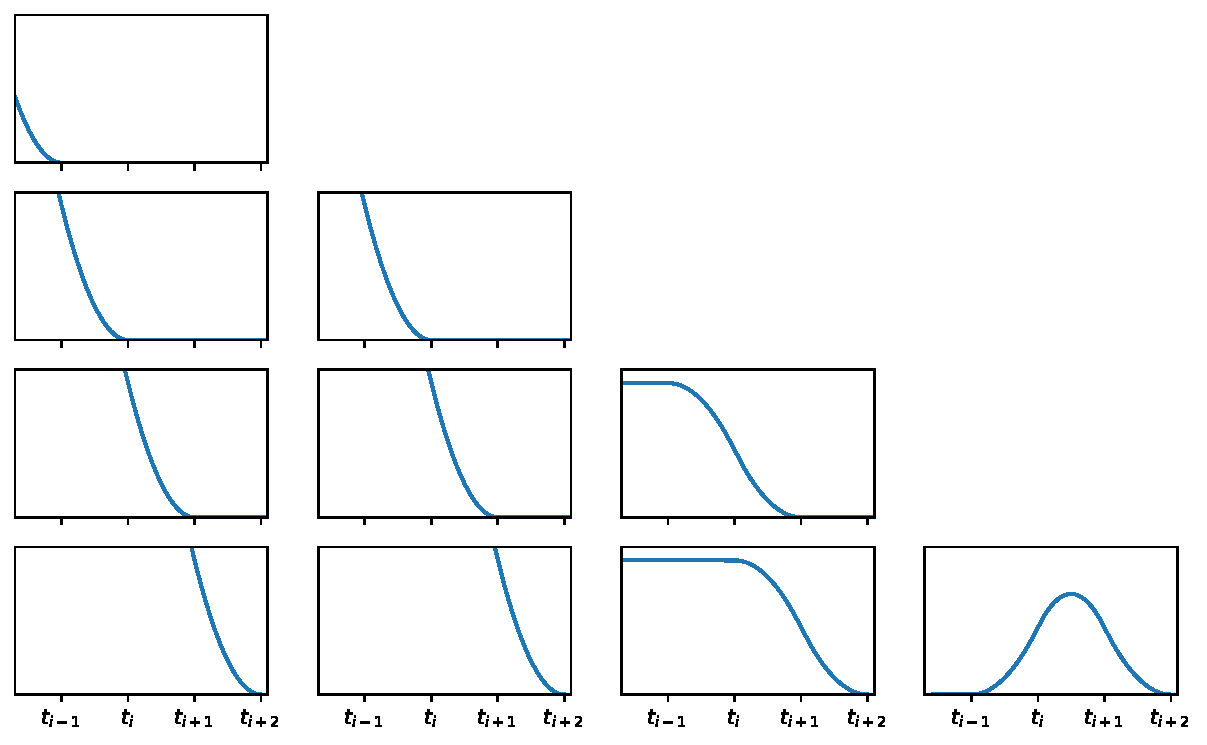
\includegraphics[scale=0.8]{pics/G_2}
        \end{figure}
        \(n=3\)
        \begin{figure}[H]
            \centering
            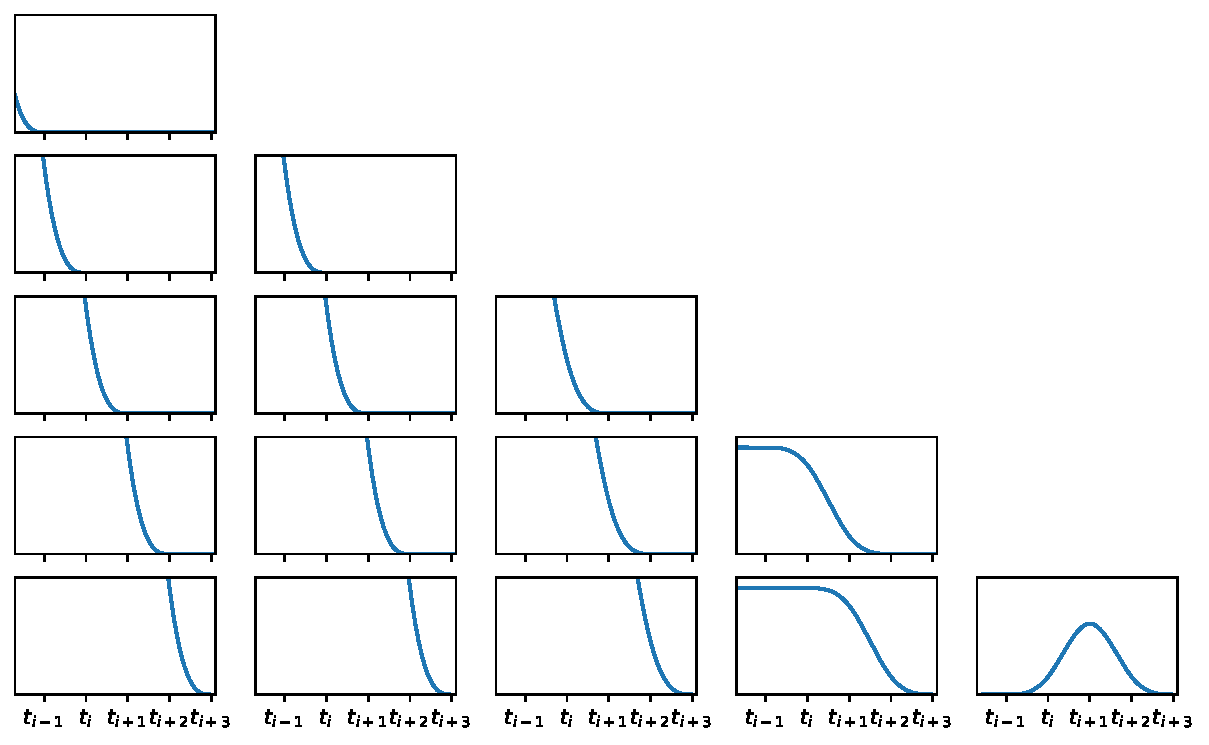
\includegraphics[scale=0.8]{pics/G_3}
        \end{figure}

\end{document}